\newpage

\section{Routing \& Mapping}

A further part of the vehicle is to log the driven route and build a map by detecting the environment.
As shown in figure \ref{route_map} the vehicle drives autonomous through an unknown environment. During the
ride all objects besides the vehicle will be detected by sensor. The driven route will be logged by
storing the events of drive like orientation changes.\\
\begin{center}
\begin{minipage}{0.45\textwidth}
\label{route_map}
\includegraphics[page=3,scale=1]{sources/mapping/example_tunnel.pdf}
\captionof{figure}{Routing \& Mapping}
\end{minipage}
\end{center}

\subsection{Detection}

\subsubsection{Routing}

\begin{minipage}{0.5\textwidth}
By the installed hardware it is possible to measure the current orientation (angle) and the current speed. These values can be used to calculate the movements of the vehicle.\\
At the start of the processes and the vehicle an initialization will be proceeded, which sets the current position on an imaginary coordinate system at the point (the coordinates) (0,0)[x,y]. From this point the movements of the vehicle will be logged by calculating every new position respectively coordinate in a list.
\end{minipage}
\begin{minipage}{0.5\textwidth}
\centering
	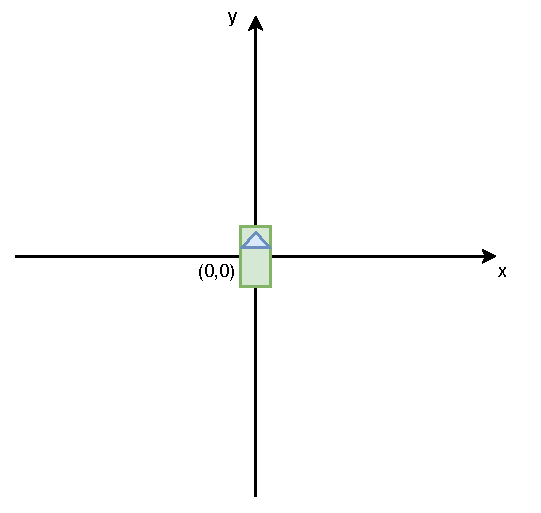
\includegraphics[scale=0.6]{sources/mapping/initial_position.pdf}
	\captionof{figure}{Initial position}
\end{minipage}

\begin{minipage}{0.5\textwidth}
\centering
	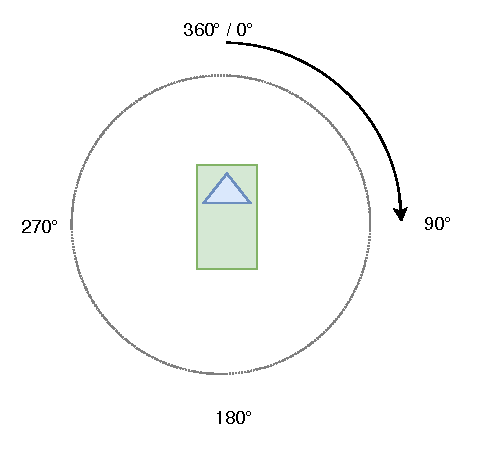
\includegraphics[scale=0.6]{sources/mapping/orientation.pdf}
	\captionof{figure}{Vehicle orientation}
\end{minipage}
\begin{minipage}{0.5\textwidth}

By using the smart movement sensor the orientation respectively the angle of the vehicle can be measured, in relation to the initial position / orientation which is 0\degree.

\end{minipage}

\begin{minipage}{0.5\textwidth}
The vehicle provides an revolution sensor by which one the current speed $v$ of the vehicle can be measured. Every time the speed changes the current time will be stored. With speed $v$ and the time slot $t$ the driven distance $s$ during this time slot can be calculated by $s=\frac{v}{t}$.
\end{minipage}
\begin{minipage}{0.5\textwidth}
	\centering
	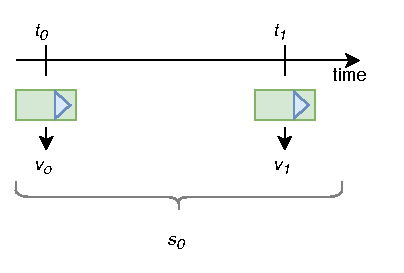
\includegraphics[scale=0.8]{sources/mapping/distance.pdf}
	\captionof{figure}{Calculated driven distance}
\end{minipage}
\\
\\
By the resulting driven distance and the orientation of the vehicle the coordinates (related to the initial position and the following positions) can be calculated. The order of these coordinates results in the driven route.

\begin{minipage}{\textwidth}
	\centering
	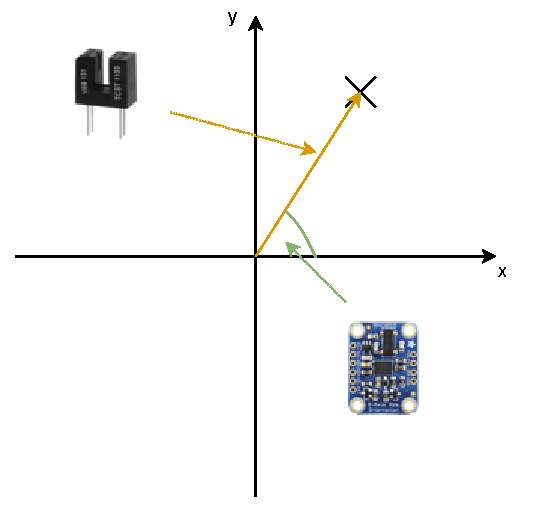
\includegraphics[scale=0.6]{sources/mapping/orientation_distance.pdf}
	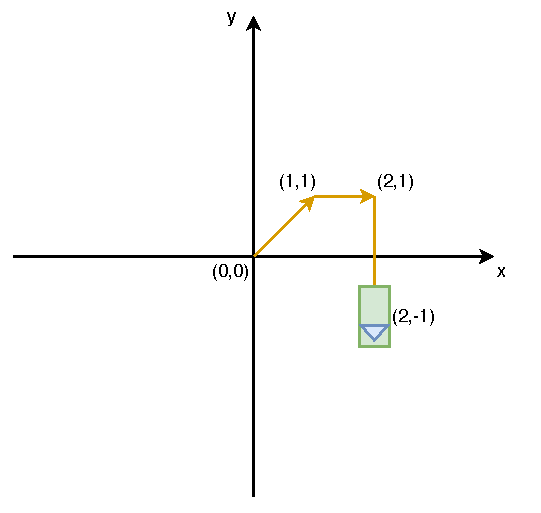
\includegraphics[scale=0.6]{sources/mapping/route.pdf}
	\captionof{figure}{Logged route information}
\end{minipage}
\\
\\
By the information of the driven route the current position of the vehicle is known.

\newpage

\subsubsection{Mapping}

To detect object around the vehicle respectively the environment ultra sonic sensors are used. On the vehicle four sensors are installed, one at the front, rear, left and right.\\
The detected objects will be also logged by coordinates in relation to the current position and orientation of the vehicle.\\
In the beginning the sensor data will be read. These data will stored in coordinates which will adjust by adding the orientation of the vehicle to calculations. Finally, the calculated coordinates will be added to the current position coordinates of the vehicle to result the object position in relation to the initial point (0,0).

\begin{center}
	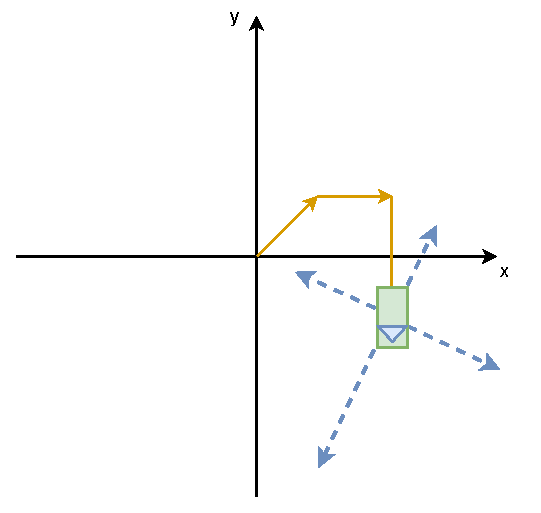
\includegraphics[page=1,scale=0.6]{sources/mapping/orientation_objectdistance.pdf}
	\includegraphics[page=2,scale=0.6]{sources/mapping/orientation_objectdistance.pdf}
	\includegraphics[page=3,scale=0.6]{sources/mapping/orientation_objectdistance.pdf}
	\captionof{figure}{Smart movement and ultra sonic sensor}
\end{center}

\newpage

\subsection{Software}

The routing \& mapping is a self-contained process as described in the beginning of this report and has been developed with Java.\\
It contains several classes which will be show following:

\begin{table}[h]
\begin{center}
	\begin{tabular}{|p{0.3\textwidth}|p{0.7\textwidth}|}
		\hline
		Class & Description\\\hline\hline
		ProcessMain & Includes the main-methode to start the process by calling the method \textit{processControl()} of the class ProcessControl. It also may be used call additional method of further classes which may be added.\\\hline
		ProcessControl & Calls the relevant methods to run the important tasks.\\\hline
		SystemData & Stores the system relevant information like port or communication codes.\\\hline
		NetworkInterface & Establishes the network communication with the navigation process.\\\hline
		LogFile & Creates and edits the log files.\\\hline
		MessageAnalysis & Checks the received messages and their contents and handles the following processing\\\hline
		MapData & Stores and handles the data for the route and map building.\\\hline
		Calculations & Offers the methods for the calculations.\\\hline
		DrawRoute & Includes the methods for the route.png to be created.\\\hline
		DrawMap & Includes the methods for the map.png to be created.\\\hline
	\end{tabular}
	\caption{Process classes}
	\end{center}
\end{table}


As described before the relevant methods for this process will be called by the method \textit{processControl()}, which is shown below. To describe this the sequence more understandably the program sequence is graphically shown in figure \ref{programSequence}

\lstset{language=Java,
   basicstyle=\small,
   keywordstyle=\color{blue!80!black!100},
   identifierstyle=,
   commentstyle=\color{green!50!black!100},
   stringstyle=\ttfamily,
   breaklines=true,
   numbers=left,
   numberstyle=\small,
   frame=single,
   backgroundcolor=\color{blue!3}
}
\lstset{language=Java}

\begin{lstlisting}
public void processControl() {
	processInitialisation();
	while(!system.endOfProcess) {
		analysis.checkMessage(network.readSocket());
	}
	System.out.println("\nBuilding route...");
	drawRoute.buildMap(mapData.routeX, mapData.routeY, "Route", routeCoordinates);
	System.out.println("route.png created.\nBuilding map...");
	drawMap.buildMap(mapData.mapX, mapData.mapY, "Map", mapCoordinates);
	System.out.println("map.png created.\n");
		
	System.out.println("System ends.");
}
\end{lstlisting}
\captionof{lstlisting}{Method \textit{processControl()}}

In the beginning an initialization process will be proceeded. This includes the establishment of the network communication with the navigation process. Also, the first data of the sensor will be received to initialize the start position of the vehicle and respectively the center of the coordinate system (0,0).\\


\begin{minipage}{0.4\textwidth}
The code of the process includes a boolean variable which will be set true, if the navigation process wants the process to be ended. This variable will check every time the while-loop start at the beginning. After this check the process waits for a message to be received in depend on the type of information to be received.\\
There are two options of informations to be received. The message could have the length of one byte, then this byte gives informations if the process has to stop, the vehicle rotates or which type of values will be send in the message. With that type of information the process knows the byte array length of the next message. \\
If the message is longer than one byte the message includes sensor data and can be directly transfer to the methods which handle value data.\\
\end{minipage}
\begin{minipage}{0.6\textwidth}
\label{programSequence}
\begin{center}
	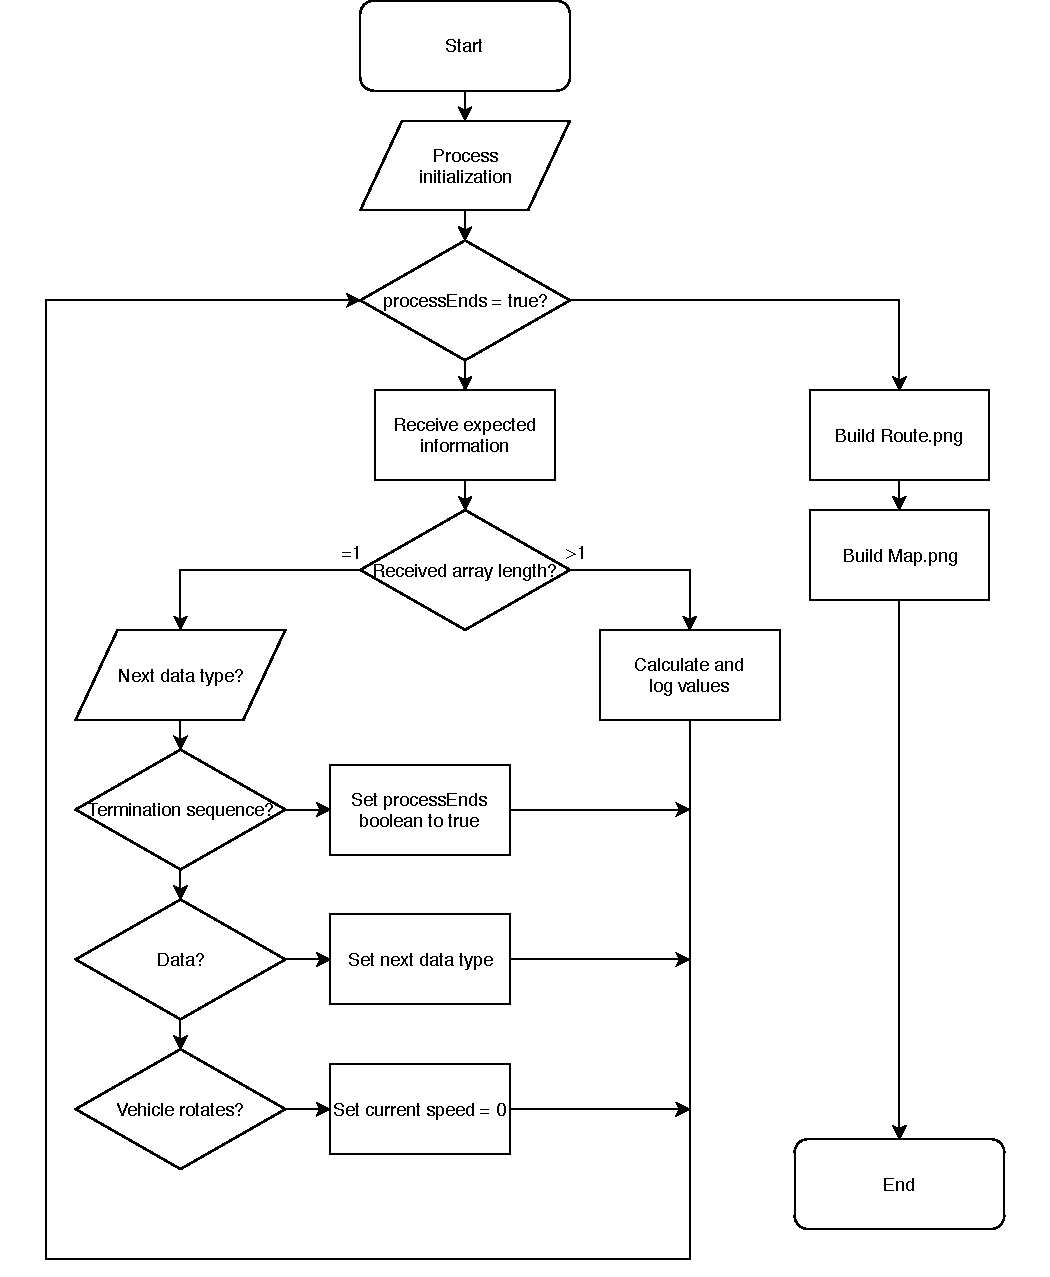
\includegraphics[scale=0.6]{sources/mapping/program_sequence.pdf}
	\captionof{figure}{Program sequence}
\end{center}
\end{minipage}

Finally the while-loop start at the beginning till the navigation process sends the termination sequence.\\
If this sequence will be received the while-loop stops and the methods to build the grphicals files for the route and the map will be called.

\begin{center}
	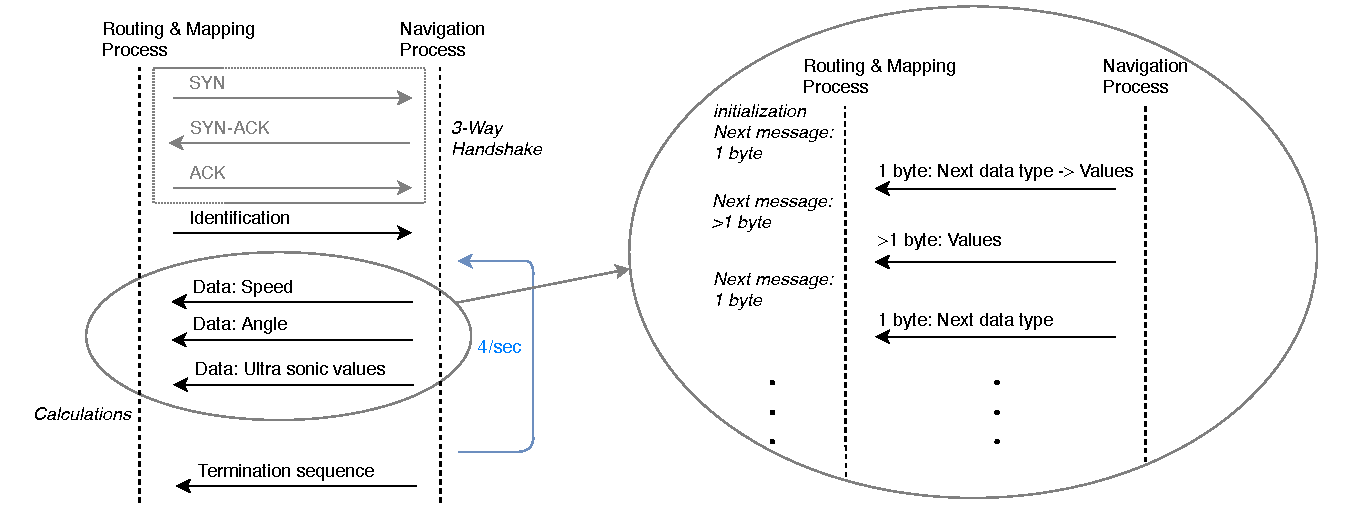
\includegraphics[scale=0.7]{sources/mapping/communication.pdf}
	\captionof{figure}{Principle commuication}
\end{center}


While the process runs all the calculated coordinates of the route and the map respectively the objects will be stored in log files. At the end of the process the classes DrawRoute and DrawMap read the named files to get the coordinates. By these coordinates the wanted .png files will be created as shown below.

\begin{minipage}{0.5\textwidth}
\begin{center}
	\includegraphics[scale=0.015]{sources/mapping/Route.png}
	\captionof{figure}{Route.png}
\end{center}
\end{minipage}
\begin{minipage}{0.5\textwidth}
\begin{center}
	\includegraphics[scale=0.015]{sources/mapping/Map.png}
	\captionof{figure}{Map.png}
\end{center}
\end{minipage}


\subsection{Problems}

Unfortunately some problems with the ultra sonic sensors occurred.\\
The measured distance of the objects are not continuously correct respectively useful. By this error it is not possible to build an adequate map. The main object which are visible in the map build the shape of the route. The object in which direction the vehicle drives will be detected several times but with kind of random values. This causes the visible shape of the route in the map.